\chapter*{易错题回顾} % {第3章校本作业}

\section*{不等式}
\begin{enumerate}
    \item 若$a,b>0$, 可得: $a+b+\dfrac{1}{\sqrt{ab}}\geq 2\sqrt{ab}+\dfrac{1}{\sqrt{ab}}\geq 2\sqrt{2\sqrt{ab}\cdot\dfrac{1}{\sqrt{ab}}}=2\sqrt2$, 
则等号成立的条件为\blkda[2.5]{$a=b=\frac{\sqrt{2}}{2}$}. 
    \item 下列各式中, 最小值为4的是\dotfill(\kh{B})
    \xx
    {$x+2\sqrt{x}+5$}
    {$\dfrac{x^2+5}{\sqrt{x^2+1}}$}
    {$x^2+3+\dfrac{4}{x^2+3}$}
    {$x+\dfrac{4}{x}$}
    \begin{jieda}
        注意取等条件是否可以取到！
    \end{jieda}
    \item
    \begin{enumerate}[(1)]
        \item 已知$x>0,y>0$, 且$2x+8y-xy=0$, 求$xy$和$x+y$的最小值; 
        \item 已知$x>0,y>0$, 且$x+y=2$, 求$x^2+y^2$的最小值. 
    \end{enumerate}
    \begin{jieda}
        \begin{enumerate}[(1)]
            \item 首先消元得到$y = \dfrac{2x}{x-8}$
            \begin{enumerate}
                \item $xy = \dfrac{2x^2}{x-8}$，转为二次比一次求最值问题。换元$t = x-8, x = t + 8$（由于$x>0, y>0$故$t > 0$）\\
                $xy = \dfrac{2(t+8)^2}{t} = 2(t + \dfrac{64}{t} + 16) \geq 64$（$t = 8$，即$x = 16, y = 4$时取等）
                \item $x+y = x + \dfrac{2x}{x-8} = 2 + x + \dfrac{16}{x-8} = 10 + (x-8) + \dfrac{16}{x-8} \geq 18$（$x = 12, y = 6$时取等）
            \end{enumerate}
            \item 
            \begin{enumerate}
                \item 方法1 \\
                消元处理$y = 2-x$，$x^2 + y^2 = x^2 + (2-x)^2 = 2x^2 - 4x + 4 = 2(x-1)^2+2 \geq 2$（$x = y = 1$时取等）
                \item 方法2 \\
                从形式上可以判断出容易平方处理.\\
                $x^2+2xy+y^2 = 4$，$x^2 + y^2 = 4 - 2xy \geq 4 - 2(\dfrac{x+y}{2})^2 = 2$ （$x = y = 1$时取等）
            \end{enumerate}
        \end{enumerate}
    \end{jieda}
    \item 若$a>b>0$, 则$a^2+\dfrac{16}{b(a-b)}$的最小值是\blkda{16}. 
    \begin{jieda}
        先考虑消元，$b(a-b) \leq \left (\dfrac{b+(a-b)}{2}\right )^2$，取等条件为$a = 2b$. \\
        故$a^2+\dfrac{16}{b(a-b)} \geq a^2 + \dfrac{64}{a^2} \geq 16$. 取等条件为$a = 2\sqrt{2}, b = \sqrt{2}$
    \end{jieda}
    \item 已知不等式$(x+y)\left(\dfrac{a}{x}+\dfrac{1}{y}\right)\geq 9$对任意正实数$x,y$恒成立, 则正实数$a$的最小值是\dotfill(\kh{B})
    \xx
    {2}
    {4}
    {6}
    {8}
    \begin{jieda}
        首先求出$(x+y)\left(\dfrac{a}{x}+\dfrac{1}{y}\right)$最小值(含$a$)，然后令其大于等于9，得到$a$的取值范围，从中选取最小值\\
        $(x+y)\left(\dfrac{a}{x}+\dfrac{1}{y}\right) = a + 1 + \dfrac{ay}{x} + \dfrac{x}{y} \geq a + 1 + 2\sqrt{a}$（$x  = \sqrt{a}y$时取等）\\
        设$f(a) = a+1+2\sqrt{a}$，显然$f(a)$单调递增，且有$f(4) = 9$. 故$a \geq 4$时原始$\geq 9$，因此$a$最小值为4.
    \end{jieda}
    \item 已知正整数$a,b$满足$4a+b=30$, 则使得$\dfrac{1}{a}+\dfrac{1}{b}$取得最小值的有序数对$(a,b)$是\dotfill(\kh{A})
    \xx
    {$(5,10)$}
    {$(6,6)$}
    {$(7,2)$}
    {$(10,5)$}
    \item ``$ab\geq 0$''是``$\abs{a+b}=\abs{a}+\abs{b}$''的\blk 条件. \dotfill(\kh{C})
    \xx
    {充分不必要条件}
    {必要不充分条件}
    {充要条件}
    {既不充分也不必要条件}
    \begin{jieda}
        考察三角不等式的取等条件. \\
        $\abs{a+b} \leq \abs{a}+\abs{b}$的取等条件是$ab\geq 0$ \\
        $\abs{a-b} \leq \abs{a}+\abs{b}$的取等条件是$ab\leq 0$
    \end{jieda}
    \item 函数$f(x) = |3-x| + |x-7|$的最小值为\blkda{$4$}.
    \begin{jieda}
        平底锅函数，可以应用三角不等式$|a|+|b| \geq |a+b|$求最小值
    \end{jieda}
    \item 若函数$f(x) = |x+1| + |2x+a|$的最小值为3，则实数$a$的值为\blkda{$-4 \mbox{或} 8$}.
    \begin{jieda}
        斜底锅函数$f(x) = |ax+b|+|cx+d|$（$|a| \neq |c|$），若$|a| > |c|$，则取最小值时$x = -\dfrac{b}{a}$，若$|a| < |c|$，则取最小值时$x = -\dfrac{d}{c}$\\
        对于本题，显然最小值在$x = -\dfrac{a}{2}$时取，因此有$|1-\dfrac{a}{2}| = 3$，故$a = -4 \mbox{或} 8$
    \end{jieda}
    \item 
    \begin{enumerate}
        \item  若关于$x$的不等式$\abs{x-1}-\abs{x-2}<a$的解集为$\bR$, 则实数$a$的取值范围为\blkda{$a>1$}
        
        \item 若关于$x$的不等式$\abs{x-1}-\abs{x-2}<a$有实数解, 则实数$a$的取值范围为\blkda{$a>-1$}. 
        
        \item 若关于$x$的不等式$\abs{x-1}-\abs{x-2}<a$的解集为$\varnothing$, 则实数$a$的取值范围为\blkda{$a\leq-1$}. 
    \end{enumerate}
    \begin{jieda}
        斜坡函数$f(x) = |x+a|-|x+b|$，最大值为$|a-b|$，最小值为$-|a-b|$. \\
        例如：$f(x) = |x+1|-|x+2| = \left \{ \begin{array}{ll}
            1 & x < -2 \\
            -2x-3 & x \in [-2, -1] \\
            -1 & x > -1 \\
        \end{array}\right.$
    \end{jieda}

    
\end{enumerate}
\section*{函数}
\begin{enumerate}
    \item 函数$f(x)=\dfrac{(x+1)^0}{\sqrt{|x|-x}}$的定义域是\blkda[3]{$(-\infty, -1) \cup (-1, 0)$}.
    \begin{jieda}
    根式里非负以及分母不为零要求$x < 0$；分子上要求$x \neq -1$，综上得到$x \in (-\infty, -1) \cup (-1, 0)$ \\
    \ps $f(x) = \dfrac{1}{\sqrt{g(x)}}$的定义域要求$g(x) > 0$.\\
    学生容易忽视分母上不为零的约束，只判断了$|x| - x \geq 0$恒成立，由此得到的答案为$(-\infty, -1) \cup (-1, 0]$
    \end{jieda}
    \item 已知函数$y=\sqrt{mx^2+(m-3)x+1}$的值域是$[0,+\infty)$, 则实数$m$的取值范围是\blkda[2.5]{$[0,1]\cup[9,+\infty)$}. 
\begin{jieda}
令$f(x)=mx^2+(m-3)x+1$, 则问题归结为$y=f(x)$在$\bR$上的值域包含$[0,+\infty)$. \\
(1) $m=0$时, 显然符合条件; \\
(2) $m\neq 0$时, 有$m>0 \mbox{且} \Delta\geq 0$, 即$m\in(0,1]\cup[9,+\infty)$. \\
综上, $m\in[0,1]\cup[9,+\infty)$. 
\end{jieda}
    \item 设函数$f(x)=\dfrac{1}{\sqrt{ax^2+ax+1}}$分别满足下列条件, 求实数$a$的取值范围: 
\begin{enumerate}
\item 定义域恰是$(-2,1)$; 
\item 定义域是$\mathbf{R}$; 
\item 值域是$(0,+\infty)$. 
\end{enumerate}
\begin{jieda}
\begin{enumerate}
    \item 定义域恰是$(-2,1)$即$ax^2+ax+1>0$的解集为$(-2,1)$. 因此对应方程$ax^2+ax+1=0$的两根为$-2, 1$，将$1$代入方程可以解得$a = -\dfrac{1}{2}$，因此$a$的取值范围是$\{-\dfrac{1}{2}\}$
    
    \item $ax^2+ax+1>0$恒成立. \\
    $a=0$时显然成立; \\
    $a\neq 0$时, $a>0$且$ \Delta<0$, 即$a\in(0,4)$. \\
    故$a\in[0,4)$. 
    
    \item 问题等价于$y=ax^2+ax+1$的值域包含$(0,+\infty)$. \\
    $a=0$显然不符合条件; \\
    $a\neq 0$时, $a>0$且$\Delta\geq0$, 即$a\geq 4$. \\
    故$a\geq 4$. \\
    \ps 学生容易犯两类错误：\\
        1. 误认为当$\sqrt{ax^2+ax+1}$的定义域是$\mathbf{R}$时，其值域是$(0, +\infty)$，从而错误地将问题转化为$\sqrt{ax^2+ax+1}$的定义域是$\mathbf{R}$，要求对应的二次函数开口向上且$\Delta < 0$，得到$[0, 4)$\\
        2. 计算$\Delta \geq 0$之后忘记开口方向的约束，得到$(-\infty, 0] \cup [4, +\infty)$
    \end{enumerate}
    \end{jieda}
    \item 已知函数$f(x)=\begin{cases}
    (x+1)^2, & x<1\\
    4-\sqrt{x-1}, & x\geq 1
    \end{cases}$, 
    则使得$f(x)\geq 1$的$x$的取值范围是\blkda[3]{$(-\infty,-2]\cup[0,10]$}. 
    \begin{jieda}
    分段函数分段求, 还要作何打算. \\
    \ps 错误率非常高
    \end{jieda}
    \clearpage
    \item 已知$f(x)=x+2, x\in[1,4]$, 则$y=f(x^2)+f^2(x)$的最大值是\blkda{22}. 
    \begin{jieda}
    先看定义域: $x\in[1,4]\land x^2\in[1,4]$, 故$x\in[1,2]$. \\
    于是$y=x^2+2+(x+2)^2=2x^2+4x+6=2(x+1)^2+4\in[12,22]$. 
    \end{jieda}
    \item 根据函数$y=f(x)$的图像: \\
    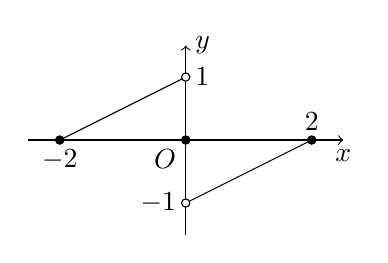
\begin{tikzpicture}
    \draw[->](-2,0)--(2,0)node[below]{$x$};
    \draw[->](0,-1.2)--(0,1.2)node[right]{$y$};
    \draw(-1.6,0)node[below]{$-2$}--(0,0.8)node[right]{1};
    \draw(1.6,0)node[above]{2}--(0,-0.8)node[left]{$-1$};
    \filldraw[fill=black](0,0)circle(1.5pt)node[below left]{$O$};
    \filldraw[fill=black](-1.6,0)circle(1.5pt);
    \filldraw[fill=black](1.6,0)circle(1.5pt);
    \filldraw[fill=white](0,0.8)circle(1.5pt);
    \filldraw[fill=white](0,-0.8)circle(1.5pt);
    \end{tikzpicture}
    \begin{enumerate}
    \item 求$y=f(x)$的解析式; 
    \item 若$g(x)=f(\frac{1}{x})$, 求$y=g(x)$的解析式, 并作出$g(x)$的图像. 
    \end{enumerate}
    \begin{jieda}
    \begin{enumerate}
    \item $f(x)=\begin{cases}
    \frac{1}{2}x+1, & x\in[-2,0)\\
    0, & x = 0 \\
    \frac{1}{2}x-1, & x\in(0,2]
    \end{cases}$. 
    
    \item $g(x)=\begin{cases}
    \frac{1}{2x}+1, & x\leq-\frac{1}{2}\\
    \frac{1}{2x}-1, & x\geq\frac{1}{2}
    \end{cases}$. \\
    \end{enumerate}
    \ps 正确率太低, 问题集中在$g(x)$的定义域上.
    \end{jieda}
    \item 若函数$f(x)=x^2-3x-4$的定义域为$[0,m]$, 值域为$\left[-\dfrac{25}{4},-4\right]$, 则实数$m$的取值范围是\blkda{$[\frac{3}{2},3]$}. 
    \begin{jieda}
    $f(x)=x^2-3x-4=(x-\frac{3}{2})^2-\frac{25}{4}$，因此$x = \dfrac{3}{2}$是函数值$-\dfrac{25}{4}$对应的唯一自变量，必然要在定义域内. 又因为$f(0)=f(3)=-4$, 是$f(x)=-4$唯二的解. 于是由二次函数的图像易得$m\in[\frac{3}{2},3]$. 
    \end{jieda}
    \item 已知函数$f(x)=\dfrac{4}{\abs{x}+2}-1$的定义域为$[a,b](a,b\zz)$, 值域是$[0,1]$, 则满足条件的整数对$(a,b)$共有\blkda{5} 对. 
    \begin{jieda}
    $f(x)\in[0,1] \iff \dfrac{4}{\abs{x}+2} \in [1, 2] \iff \dfrac{1}{\abs{x}+2} \in [\dfrac{1}{4}, \dfrac{1}{2}] \iff \abs{x}+2 \in [2, 4] \iff \abs{x}\in[0,2] \Leftarrow  x\in[-2,2]$. \\
    分析函数的性质：首先判断函数$y = |x|$ 为偶函数，在$[-2, 0]$单调增，在$[0, 2]$单调减。\\
    $x = 0$是函数值$1$对应的唯一自变量，$x = 2 \mbox{或} -2$是函数值$0$对应的唯二自变量，故有: \\
    若$a=-2$, 则$b=0,1,2$; 若$b=2$, 则$a=-2,-1,0$. \\
    列举、排除重复情况可得所求为5. 
    \end{jieda}
    \item 若一系列函数的解析式相同, 值域相同, 但其定义域不同, 则称这些函数为``同族函数'', 
    那么函数解析式为$f(x)=x^2$, 值域为$\{1,4\}$的``同族函数''共有\blkda{$9$}个.
    \begin{jieda}
    $1,-1,\pm1\to 1$, $2,-2,\pm2\to 4$, 于是从值域的角度, $x$的组合共有$3\times3=9$种选择. \\
    \ps 此题错误率非常高，分成两种情况。1. 学生没有乘法原理的概念，采用列举法时候出错；2. 学生忽视可以取两个自变量对应于一个函数值的情况。
    \end{jieda} 
    \item 设$f(x)$和$g(x)$分别是$\mathbb{R}$上的偶函数和奇函数, 则下列结论恒成立的是\dotfill(\kh{A})
    \xx{$f(x)+\abs{g(x)}$是偶函数}{$f(x)-\abs{g(x)}$是奇函数}{$\abs{f(x)}+g(x)$是偶函数}{$\abs{f(x)}-g(x)$是奇函数}
    \begin{jieda}
    $g(x)$为奇函数，则$|g(x)|$为偶函数，偶函数$+$偶函数还是偶函数，故$A, B$都是偶函数，$A$正确，$B$错误。\\
    $f(x)$是偶函数，$|f(x)|$还是偶函数。奇函数$+$偶函数的结果是不确定的（如果两个函数都不是“既是奇函数又是偶函数”的话，结果必然非奇非偶函数）。故$C,D$都错。\\
    \ps 任意一个关于定义域关于原点对称的函数都可以写成一个奇函数加上一个偶函数（包含其中之一为既奇又偶的情况）：$h(x) = \dfrac{h(x)+h(-x)}{2} + \dfrac{h(x) - h(-x)}{2}$
    \end{jieda}
    
    \item 函数$f(x)=x\abs{x+a}+b$是奇函数的充要条件是\dotfill(\kh{B})
    \xx{$ab=0$}{$a^2+b^2=0$}{$a=b$}{$a+b=0$}
    \begin{jieda}
    奇函数若在$x=0$处有定义, 则此处的函数值为零, 即$f(0)=0$, 于是$b=0$. \\
    故$f(x)=x\abs{x+a}$. 于是由$f(x)$为奇函数，不难得到$a=0$, 比如$f(-a)+f(a)=0$. 
    \end{jieda}
    \item 已知函数$f(x)=x^5+ax^3+bx-8$, 且$f(-2)=10$, 则$f(2)$=\blkda{$-26$}
    \begin{jieda}
    $f(x)+f(-x)=-16$，函数关于$(0, -8)$中心对称。\\
    \ps 设$g(x) = f(x)+8$，则$g(x)$为奇函数. (多项式函数是奇函数等价于偶次方的系数为零, 是偶函数等价于奇次方的系数为零.)
    \end{jieda}
    \item 定义在 $[-1,1]$ 上的奇函数 $f(x)$ 满足 $f(1)=2$, 且当 $a, b \in[-1,1], a+b \neq 0$ 时,有 $\dfrac{f(a)+f(b)}{a+b}>0$.
    \begin{enumerate}
        \item 判定函数 $f(x)$ 在 $[-1,1]$ 的单调性并加以证明;
        \item 若 $\dfrac{1}{2} f(x) \leq m^2+2 a m+1$ 对所有 $x \in[-1,1], a \in[-1,1]$ 恒成立, 求 $m$ 的取值范围.
    \end{enumerate}
    \begin{jieda}
        \begin{enumerate}
            \item 将$\dfrac{f(a)+f(b)}{a+b}>0$中的$b$代换为$-b$有$\dfrac{f(a)+f(-b)}{a-b}>0$，根据$f(x)$是奇函数，可以转化为$\dfrac{f(a)-f(b)}{a-b}>0$，由此可以判断出$f(x)$在$[-1, 1]$上单调增。 \\
            证明略.
            \item 不等式左侧的最大值要小于右侧，因为$f(x)$单调增，所以不等式左侧最大值为$\dfrac{1}{2}f(1) = 1$，由此不等式转化为$0 \leq m^2 + 2am$在$a \in [-1, 1]$恒成立。设$g(a) = 2ma+m^2$，故应有$g(-1) \geq 0, g(1) \geq 0$，因此$m \in (-\infty, -2] \cup [2, +\infty) \cup \{0\}$
        \end{enumerate}
    \end{jieda}
    \item 已知函数$y=f(x)$是$\mathbb{R}$上的不恒为0的函数, 且对于任意的$a,b\zr$, 都有$f(ab)=af(b)+bf(a)$；
    \begin{enumerate}
        \item 求$f(0), f(1)$的值；
        \item 判断$y=f(x)$的奇偶性，并证明你的结论. 
    \end{enumerate}
    \begin{jieda}
    容易判断出应该利用迭代法解决问题，首先考虑带入常值特值。令$a=b=0$, 则$f(0)=0$. 令$a=b=1$, 则$f(1)=0$. 令$a=1, b=-1$, 则$f(-1)=0$. \\
    下一步为了判断奇偶性，应当考虑得到$-x$的形式，故令$a=-1$, $b=x$, 则对任意$x$有$f(-x)=-f(x)+xf(-1)=-f(x)$. 故$f(x)$是奇函数. \\
    又不恒为0, 故仅是奇函数. 
    \end{jieda}
    \item 函数$y=-(x-3)\abs{x}$的严格单调增区间是\blkda{$[0,\frac{3}{2}]$}. 
    \begin{jieda}
    $f(x)=(x-a)\abs{x-b}$的图像如何? 数形相结合之后, 数形皆可作为判断单调区间的方法, 只不过``形'' 最好不要作为证明的唯一依据. \\
    \ps 解析式中有部分绝对值，要考虑分类讨论，写成分段函数. \\
    \ps 错误率高.
    \end{jieda}
    \item 函数 $f(x)=\frac{1}{\sqrt{x^2-8 x+15}}$ 的单调减区间是\blkda{$(5,+\infty)$}.
    \item 已知函数$f(x)=2x-\dfrac{a}{x}, x\in(0,1]$是严格减函数, 求实数$a$的取值范围. 
    \begin{jieda}
    设$0<x_1<x_2\leq 1$, 则$f(x_2)-f(x_1)=(x_2-x_1)\cdot\dfrac{2x_1x_2+a}{x_1x_2}<0$恒成立. \\
    于是$a<-2x_1x_2$恒成立. \\
    因为$0<x_1<x_2\leq 1$, 则$-2x_1x_2\in(-2,0)$, 故$a\leq -2$. \\
    \ps 对$a$分类讨论是一种解法, 这里写一个运用定义的解法, 关键在于恒成立与等号能否成立. 
    \end{jieda}
    \item 已知函数 $f(x)=\left\{\begin{array}{l}x^{2}+2 a x, x \geq-1 \\ (2-a) x+2 a-5, x<-1\end{array}\right.$, 若 $f(x)$ 在 $\mathbf{R}$ 上是增函数, 则实数 $a$ 的取值范围是\blkda{$1 \leq a \leq \frac{8}{5}$} .
    \begin{jieda}
    由函数 $f(x)=\left\{\begin{array}{l}x^{2}+2 a x, x \geq-1 \\ (2-a) x+2 a-5, x<-1\end{array}\right.$ 在 $\mathbf{R}$ 上是增函数, 得 $\left\{\begin{array}{l}-a \leq-1 \\ 2-a>0 \\ 1-2 a \geq-(2-a)+2 a-5\end{array}\right.$,解得 $1 \leq a \leq \frac{8}{5}$,
    所以实数 $a$ 的取值范围是 $1 \leq a \leq \frac{8}{5}$.
    故答案为: $1 \leq a \leq \frac{8}{5}$
    \end{jieda}
    
    \item 已知 $x>0, y>0$ ，若 $\sqrt{4 x^{2}+3 x y+y^{2}}+m \sqrt{x y}>2 x+y$ 恒成立，则实数 $m$ 的取值范围是\blkda[3]{$(2 \sqrt{2}-\sqrt{7},+\infty)$}.
    \begin{jieda}
    原不等式等价于 $m>\dfrac{2 x+y-\sqrt{4 x^{2}+3 x y+y^{2}}}{\sqrt{x y}}$,令 $z=\dfrac{2 x+y-\sqrt{4 x^{2}+3 x y+y^{2}}}{\sqrt{x y}}=2 \sqrt{\frac{x}{y}}+\sqrt{\frac{y}{x}}-\sqrt{4 \frac{x}{y}+\frac{y}{x}+3}$.令 $t=2 \sqrt{\frac{x}{y}}+\sqrt{\frac{y}{x}}$, 且 $t \geq 2 \sqrt{2}$,则 $z=t-\sqrt{t^{2}-1}=\frac{1}{t+\sqrt{t^{2}-1}}$ 在 $(2 \sqrt{2},+\infty)$ 上单调减, $\therefore z \leq \frac{1}{2 \sqrt{2}+\sqrt{7}}=2 \sqrt{2}-\sqrt{7}, \therefore m>2 \sqrt{2}-\sqrt{7}$.
    故 $m$ 的范围是 $(2 \sqrt{2}-\sqrt{7},+\infty)$.
    故答案为: $(2 \sqrt{2}-\sqrt{7},+\infty)$ \\
    \ps $z = t - \sqrt{t^2-1}$（$t > 0$）可以看做$z = \sqrt{t^2} - \sqrt{t^2-1}$，这样的两个齐次且对应系数相同的根式相减可以通过分子有理化使得分子为常数，分母上为容易判断单调性的形式.
    \end{jieda}
    \item 已知函数 $f(x)=\frac{\sqrt{2021-a x}}{a-1}$ 在 $[0,1]$ 上严格单调减，那么实数 $a$ 的取值的范围是\blkda[3]{$(-\infty, 0) \cup(1,2021]$}.
    \begin{jieda}
    当 $a<0$ 时, $y=\sqrt{2021-a x}$ 在 $[0,1]$ 上单调增, 且 $a-1<0$,所以 $f(x)$ 在 $[0,1]$ 上单调减, 符合题意,\\
    当 $a=0$ 时, $f(x)=-\sqrt{2021}$ 无单调性, 不符合题意,\\
    当 $0<a<1$ 时, $y=\sqrt{2021-a x}$ 在 $[0,1]$ 上单调减, 且 $a-1<0$, 不符合题意,\\
    当 $a>1$ 时, $y=\sqrt{2021-a x}$ 在 $[0,1]$ 上单调减, $a-1>0$, 符合题意,\\
    还需 $\left\{\begin{array}{l}2021-0 \times a \geq 0 \\ 2021-1 \times a \geq 0\end{array}\right.$ ，解得 $1<a \leq 2021 ，$\\
    综上实数 $a$ 的取值的范围是 $(-\infty, 0) \cup(1,2021]$.
    \end{jieda}
    \clearpage
\item 设$a$为实数, 函数$f(x)=x^2+|x-a|+1$，设$g(a)$为函数$f(x)$的最小值，求$g(a)$最小值.
\begin{jieda}
    函数内部分含有绝对值的形式需要通过分类讨论写成分段函数的形式. \\
    $f(x) = \left \{ \begin{array}{cc}
        x^2-x+a+1 & x < a \\
        x^2+x-a+1 & x \geq a
    \end{array} \right.$ \\
    函数图象由两个二次函数图象的部分拼接而成，且拼接处连续，分析两个开口向上的二次函数的对称轴可知，一个为$x = \dfrac{1}{2}$，一个为$-\dfrac{1}{2}$ \\
    讨论拼接点$x = a$与两个对称轴不同的位置关系下函数的单调性，即可得到函数的最小值，在不同的拼接点条件下寻找全局的最小值即为$g(a)$. 
    \begin{enumerate}
        \item $a < -\dfrac{1}{2}$，此时第一段上函数单调减，第二段上先减后增，因此在第二段的顶点处取得最小值。故$g(a) = \dfrac{3}{4}-a > \dfrac{5}{4}$
        \item $a \in [-\dfrac{1}{2}, \dfrac{1}{2}]$，此时第一段上函数单调减，第二段上单调增，在$x = a$处取最小值。故$g(a) = a^2 + 1 \geq 1$（在$a$ = 0时取等）
        \item $a > \dfrac{1}{2}$，此时第一段上函数先减后增，第二段上单调增，因此在第一段的顶点处取得最小值。故$g(a) = \dfrac{3}{4}+a > \dfrac{5}{4}$
    \end{enumerate}
    综上，$g(a)$最小值为1.
\end{jieda}
\item 设$a$为实数, 函数$f(x)=2x^2+(x-a)\abs{x-a}$. 
\begin{enumerate}[(1)]
\item 若$f(0)\geq 1$, 求$a$的取值范围; 
\item 求$f(x)$的最小值. 
\end{enumerate}
\begin{jieda}
\begin{enumerate}[(1)]
\item $f(0)=-a\abs{a}$，因为$g(x)=-x\abs{x}$在$\bR$上严格单调递, 且$g(-1)=1$. \\
于是$f(0)=-a\abs{a}\geq 1=g(-1)\iff a\leq -1$.  \\
\ps 想象一下$g(x)=-x\abs{x}$的图象.


\item $f(x)=\begin{cases}
x^2+2ax-a^2, & x\leq a\\
3x^2-2ax+a^2, & x\geq a
\end{cases}$. \\
函数图象由两个二次函数图象的部分拼接而成，且拼接处连续，分析两个开口向上的二次函数的对称轴可知，一个为$x = -a$，一个为$\dfrac{a}{3}$ \\
讨论拼接点$x = a$与两个对称轴不同的位置关系下函数的单调性，即可得到函数的最小值，在不同的拼接点条件下寻找全局的最小值即为所求. 
\begin{enumerate}
    \item $a = 0$时，三者重合，此时最小值为$0$ 
    \item $a > 0$时，$-a < \dfrac{a}{3} < a$，故函数$f(x)$在第一段上先减后增，在第二段上单调增，因此最小值在第一段的顶点处取得（$x = -a$），最小值为$-2a^2$
    \item $a < 0$时，$a < \dfrac{a}{3} < -a$，故函数$f(x)$在第一段上单调递减，在第二段上先减后增，因此最小值在第二段顶点取得（$x = \dfrac{a}{3}$），最小值为$\dfrac{2a^2}{3}$
\end{enumerate}
综上，$a < 0$时为$\dfrac{2a^2}{3}$，$a \geq 0$时，$f(x)$的最小值为$-2a^2$. \\
\ps 最值需要通过单调性来说明，分段函数分段求，分析各段上函数的单调性.
另外, 本题的另一个麻烦之处在于函数中的分段点与参数$a$有关, 各段中的``对称轴''(单调区间的端点)亦与参数$a$有关. 
\end{enumerate}
\end{jieda}
\clearpage
\item 求下列函数的值域: 
\begin{enumerate}
\item $y=\dfrac{3+x}{4-x}$; 
\item $y=\dfrac{2x^2-2x+3}{x^2-x+1}$; 
\item $y=\dfrac{x^4+x^2+5}{(x^2+1)^2}$; 
\item $y=x+4\sqrt{1-x}$; 
\item $y=\dfrac{\sqrt{x^2+1}}{x-1}$. 
\item $\sqrt{1+x} - \sqrt{2+x}$.
\end{enumerate}
\begin{jieda}
\begin{enumerate}
\item $y=-1+\dfrac{7}{4-x}\in(-\infty,-1)\cup(-1,+\infty)$. 

\item $y=2+\dfrac{1}{x^2-x+1}$. \\
因为$x^2-x+1\in[\frac{3}{4},+\infty)$, 故$y\in(2,\frac{10}{3}]$. 

\item $y=\dfrac{x^4+2x^2+1+4-x^2}{x^4+2x^2+1}=1+\dfrac{4-x^2}{x^4+2x^2+1}$. \\
令$t=4-x^2$. 当$t\in(-\infty,0)\cup(0,4]$, 则$t+\dfrac{25}{t}-10\in(-\infty,-20]\cup[\frac{1}{4},+\infty)$. \\
于是当$t\leq 4$时, $y=\dfrac{t}{(t-5)^2}\in[-\frac{1}{20},4]$. \\
所以$y=1+\dfrac{4-x^2}{x^4+2x^2+1}\in[\frac{19}{20},5]$. \\
\ps 可化为$ax+\frac{b}{x}$的. 

\item 令$t=\sqrt{1-x}\in[0,+\infty)$, 则$x=1-t^2$, 故$y=1-t^2+4t=-(t-2)^2+5\in(-\infty,5]$. \\
\ps 可化为二次的. 

\item 当$x>1$时, $y=\sqrt{\dfrac{x^2+1}{x^2-2x+1}}=\sqrt{1+\dfrac{2x}{x^2-2x+1}}=\sqrt{1+\dfrac{2}{x+\frac{1}{x}-2}}\in(1,+\infty)$. \\
当$x<1$时, $y=-\sqrt{\dfrac{x^2+1}{x^2-2x+1}}=-\sqrt{1+\dfrac{2x}{x^2-2x+1}}$. \\
再分为$(-\infty,0)\cup\{0\}\cup(0,1)$讨论可得$y\in(-\infty,-\frac{1}{\sqrt{2}}]$. \\
综上, $y\in(-\infty,-\frac{1}{\sqrt{2}}]\cup(1,+\infty)$. \\
\ps 可化为$ax+\frac{b}{x}$的. \\
\ps 对于$f(x)=\dfrac{x}{x^2+1}$而言, 在$(-\infty,-1]$上$\searrow$, 在$[-1,1]$上$\nearrow$, 在$[1,+\infty)$上$\searrow$. \\
\ps 三角换元: 令$x=\tan\theta$, 其中$\theta\in(-\frac{\pi}{2},\frac{\pi}{4})\cup(\frac{\pi}{4},\frac{\pi}{2})$. \\
于是$y=\dfrac{\sec\theta}{\tan\theta-1}=\dfrac{1}{\sin\theta-\cos\theta}=\dfrac{1}{\sqrt{2}\sin(\theta-\frac{\pi}{4})}$. % (虎兕入柙)
\item $y = \sqrt{1+x} - \sqrt{2+x} = \dfrac{(\sqrt{1+x} + \sqrt{2+x})(\sqrt{1+x} - \sqrt{2+x})}{(\sqrt{1+x} + \sqrt{2+x})} = \dfrac{-1}{(\sqrt{1+x} + \sqrt{2+x})}$ \\
易知函数在定义域$[-1, +\infty)$内单调递增，最小值在左端点$x = -1$取$y = -1$，当$x$趋于无穷时，函数值趋于0。因此值域为$[-1, 0)$
\end{enumerate}
\end{jieda}
\end{enumerate}